\chapter{Konzeptionierung}
\label{ch: Konzeptionierung}

	
	
	\section{Anforderungserhebung mit CONSENS}
	\label{sec: Anforderungserhebung}
			
	
	\section{Konzept und Aufbau der Personenerkennung}
	
		\subsection{Wirkstruktur der Personenerkennung}
		
		\subsection{Auswahl und Training der verwendeten neuronalen Netze}
		
		\subsection{Entwickeltes neuronales Netz}
		\tikzset{%
			every neuron/.style={
				circle,
				draw,
				minimum size=1cm
			},
			neuron missing/.style={
				draw=none, 
				%scale=4,
				%rotate=90,
				%yshift=1,
				%text height=0.333cm,
				%execute at begin node=\color{black}$\cdots$
			},
		}
		\begin{figure}[H]
			\centering
				
				
				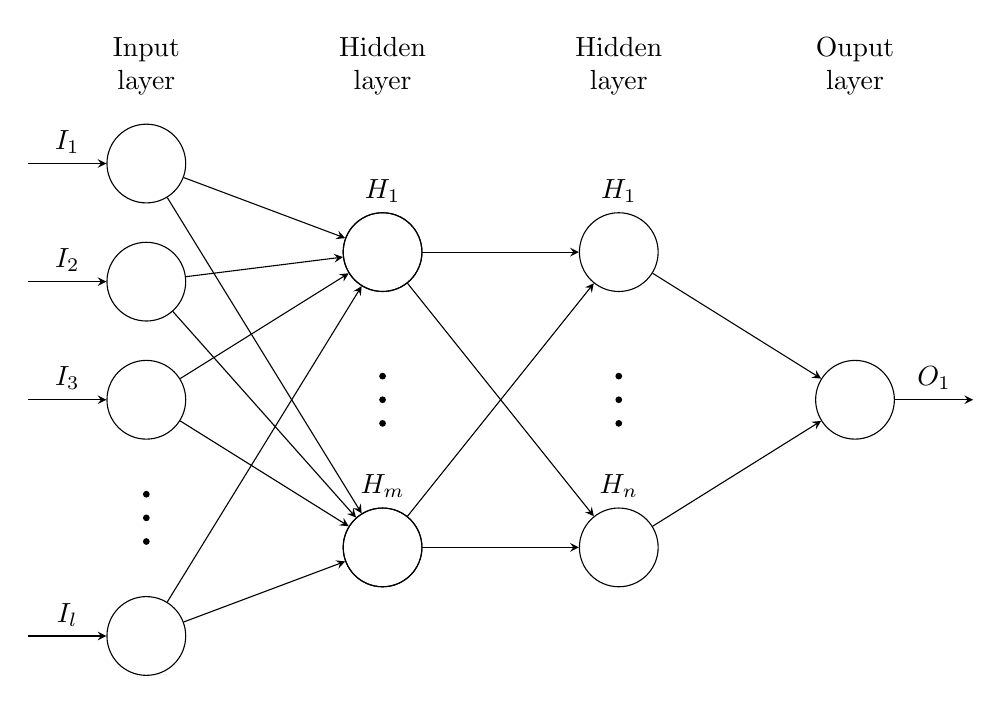
\begin{tikzpicture}[x=1.5cm, y=1.5cm, >=stealth]
					
					\foreach \m/\l [count=\y] in {1,2,3,missing,4}
					\node [every neuron/.try, neuron \m/.try] (input-\m) at (0,2.5-\y) {};
					
					\foreach \m [count=\y] in {1,missing,2}
					\node [every neuron/.try, neuron \m/.try ] (hidden1-\m) at (2,2-\y*1.25) {};
					
					\foreach \m [count=\y] in {1,missing,2}
					\node [every neuron/.try, neuron \m/.try ] (hidden1-\m) at (2,2-\y*1.25) {};
					
					\foreach \m [count=\y] in {1,missing,2}
					\node [every neuron/.try, neuron \m/.try ] (hidden2-\m) at (4,2-\y*1.25) {};
					
					\foreach \m [count=\y] in {1}
					\node [every neuron/.try, neuron \m/.try ] (output-\m) at (6,0.5-\y) {};
					
					\foreach \l [count=\i] in {1,2,3,l}
					\draw [<-] (input-\i) -- ++(-1,0)
					node [above, midway] {$I_\l$};
					
					\foreach \l [count=\i] in {1,m}
					\node [above] at (hidden1-\i.north) {$H_\l$};
					
					\foreach \l [count=\i] in {1,n}
					\node [above] at (hidden2-\i.north) {$H_\l$};
					
					\foreach \l [count=\i] in {1}
					\draw [->] (output-\i) -- ++(1,0)
					node [above, midway] {$O_\l$};
					
					\foreach \i in {1,...,4}
					\foreach \j in {1,...,2}
					\draw [->] (input-\i) -- (hidden1-\j);
					
					\foreach \i in {1,...,2}
					\foreach \j in {1,...,2}
					\draw [->] (hidden1-\i) -- (hidden2-\j);
					
					\foreach \i in {1,...,2}
					\foreach \j in {1}
					\draw [->] (hidden2-\i) -- (output-\j);
					
					\foreach \l [count=\x from 0] in {Input, Hidden, Hidden, Ouput}
					\node [align=center, above] at (\x*2,2) {\l \\ layer};
					\draw[fill=black](0,-1.3)circle(1pt);
					\draw[fill=black](0,-1.5)circle(1pt);
					\draw[fill=black](0,-1.7)circle(1pt);
					\draw[fill=black](2,-0.3)circle(1pt);
					\draw[fill=black](2,-0.5)circle(1pt);
					\draw[fill=black](2,-0.7)circle(1pt);
					\draw[fill=black](4,-0.3)circle(1pt);
					\draw[fill=black](4,-0.5)circle(1pt);
					\draw[fill=black](4,-0.7)circle(1pt);
					
				\end{tikzpicture}
		
		\caption{https://tex.stackexchange.com/questions/132444/diagram-of-an-artificial-neural-network}
		\end{figure}
		\subsection{Schnittstelle zwischen Python und ROS}
		
		\subsection{Erstellung von Objektinformationen}
		\label{subsec: Erstellung von Objektinformationen}
	
	\section{Funktionsweise des Gesamtsystems}
	Der Kern dieser Arbeit ist die Personenerkennung im praktischen Kontext des im Kapitel ... beschriebenen autonomen Logistikfahrzeugs. Aufgrund dessen sind einzelne Programme nicht als abgeschlossenes System zu betrachten. In Kapitel .../consens wurden bereits alle Schnittstellen zu verbauten Hardware- und Softwarekomponenten präsentiert. Das vollständige System der Personenerkennung und der Aufbau des entwickelten, endlichen Automats wird im folgenden Kapitel erklärt.\\
	
	Die Personenerkennung am ALF wird mithilfe der Bildinformationen von zwei \textit{Kinect}-Kameras betrieben. In Kapitel.../rospython wurden bereits zwei Lösungsansätze in der Softwarentwicklung in Zusammenspiel mit ROS und Python präsentiert. Aufgrund einer starken Belastung der im Roboter verbauten Recheneinheit während der parallelen Bildverarbeitung beider eingehender Bilder, wurde das Programm auf eine serielle Verarbeitung umgestellt. Der Befehl der parallelen Verarbeitung erzwingt Berechnungsprozesse mit derselben Frequenz, die durch den Eingang der Bilder beider Kameras vorgegeben wird. Mithilfe der seriellen Abarbeitung  war es ebenfalls möglich die Häufigkeit der Berechnungen zu steuern und damit verbundene Programmoptimierungen vorzunehmen. Auslastungen des verbauten Computers können so eingespart werden und für weitere, parallel laufende Prozesse genutzt werden. Dies wird zum Beispiel durch eine gezielte Verzögerung der Personenerkennung erreicht. Hierbei werden Pausen mit der gewünschten Dauer zwischen Bildverarbeitungsprozessen eingelegt bis ein relevantes Bild erkannt wird. Erst dann arbeitet die Personenerkennung mit der maximalen Geschwindigkeit. Als relevant werden Bilder eingestuft, die eine Person enthalten.\\
	
	\begin{figure}[H]
		\centering
		\begin{tikzpicture}
			\node[circle,fill,gray,minimum size=15mm] (head) {};
			\node[rounded corners=2pt,minimum height=5cm,gray,minimum width=1.5cm,fill,below = 1pt of head] (body) {};
			\draw[line width=3.8mm,gray,round cap-round cap] ([shift={(6pt,-1pt)}]body.north east) --++(-90:19mm);
			\draw[line width=3.8mm,gray,round cap-round cap] ([shift={(-6pt,-1pt)}]body.north west)--++(-90:19mm);
			\draw[thick,white,-round cap] (body.south) --++(90:18mm);
			\node at (0,-2.5) [thick,dashed,rectangle,minimum height=7cm,minimum width=4cm,draw] (v100) {};
			\node at (0,-0.6) [thick,dashdotted,rectangle,minimum height=3cm,minimum width=3.8cm,draw] (v100) {};
			\node at (0,-0.0) [thick,rectangle,minimum height=1.6cm,minimum width=1.6cm,draw] (v100) {};
			
		\end{tikzpicture}
		\caption{test}
		\label{fig: bbox}
	\end{figure}

	In Abbildung \ref{fig: bbox} wird der Ablauf der Personenerkennung in Form eines Programmablaufplans dargestellt. Die Darstellung zeigt die Funktionsweise des Programms ab dem Zeitpunkt, an dem eine Person vor der jeweiligen Kamera detektiert wird. Weiterhin zeigt die Abbildung den Informationsfluss eines Bildes von einer Kamera durch die Personenerkennung. Zu Beginn der Analyse gelangt jedes Bild zunächst in das eingestellte künstliche neuronale Netz. Je nach Anzahl der erkannten Person werden korrespondierende Koordinaten ausgegeben, die die Position des Interessensbereich beschreiben. Anhand dieser Informationen kann an eine Aussage darüber getroffen werden, ob eine Person im Bild zu sehen ist und wo sich diese befindet. Wird keine Person erkannt arbeitet das Programm wieder reduziert, wie bereits beschrieben. Sollten jedoch Personen erkannt worden sein, wird versucht ein Gesicht zu erkennen. In den meisten Fällen sitzen und stehen Menschen aufrecht. So kann davon ausgegangen werden, dass sich das Gesicht einer Person im oberen Teil des Bereichs befindet. Dafür wird der Interessensbereich verkleinert, um Rechenkapazitäten einzusparen. Sollte sich kein Gesicht im relevanten Bereich befinden, wird davon ausgegangen, dass die Person stark von der Kamera abgewandt ist. Somit ist keine eindeutige Identifikation möglich und das Programm schaltet in den reduzierten Modus. Detektiert das Netz ein Gesicht wird eine Merkmalsextraktion durchgeführt.\\
	
	Im Anschluss werden die extrahierten Merkmale mit den der bereits abgespeicherten Gesichtern verglichen. Wird kein übereinstimmendes Gesicht gefunden versucht die Software das Gesicht zu registrieren. Je nach Einstellung wird ein Gesicht registriert, wenn es entsprechend oft hintereinander erkannt worden ist. Der Registrierungsprozess und die Sammlung von Bildinformationen wird in Kapitel \ref{subsec: Erstellung von Objektinformationen} behandelt. Im Falle der Erkennung eines bekannten Gesichts wird die Informationen der erkannten Person wie im bereits erwähnten Kapitel aktualisiert.\\ 
	
	  
	\newpage
	\begin{figure}[H]
		\centering
		\begin{tikzpicture}[node distance = 2cm, auto]
			
			% Place nodes
			\node [papStart] (Start1){Start};
			\node [papProcess, below of = Start1,label={[shift={(5,-0.6)}]\footnotesize\textit{Aktuelles Bild wird mit KNN analysiert}}] (pro1){Prozess};
			\node [papDecision, below of = pro1, yshift= -9mm,label={[shift={(2.7,-0.6)}]\footnotesize\textit{Menschen im Bild?}}](dec1){Entscheidung};
			\node [papProcess, right of = dec1,xshift=25mm,label={[shift={(5,-0.6)}]\footnotesize\textit{Gesichter im Interessensbereich detektieren}}](pro3){Prozess};
			\node [papDecision, below of = pro3, yshift= -9mm,label={[shift={(5,-0.6)}]\footnotesize\textit{Gesicht im Interessenbereich?}}](dec2){Entscheidung};
			\node [papProcess, below of = dec2, yshift= -9mm,label={[shift={(5,-0.6)}]\footnotesize\textit{Merkmalsextraktion des Gesichts}}](pro4){Prozess};
			\node [papDecision, below of = pro4, yshift= -9mm,label={[shift={(5,-0.6)}]\footnotesize\textit{Gesicht bekannt?}}](dec3){Entscheidung};
			\node [papDecision, below of = dec3, yshift= -18mm,label={[shift={(5,-0.6)}]\footnotesize\textit{Dasselbe unbekannte Gesicht oft genug hintereinander erkannt?}}](dec4){Entscheidung};
			\node [papProcess, below of = dec4, yshift= -9mm,label={[shift={(5,-0.6)}]\footnotesize\textit{Eigenschaften des Objekts vom Typ Mensch aktualisieren}}](pro5){Prozess};
			%\node [papData, right of = dec3, xshift= 25mm,label={[shift={(5,-0.6)}]\footnotesize\textit{Gesicht bekannt?}}](dat1){I/O};
			\node [papEnd, below of = dec1, yshift= -40mm] (End) {Ende};
			
			% Place joins
			\coordinate [below of = dec1, yshift= -9mm] (join1);
			
			% Draw edges
			\path [papLine] (Start1) -- (pro1);
			\path [papLine] (pro1) -- (dec1);
			\path [papLine] (dec1) -- node [above] {\papYes} (pro3);
			\draw (dec1) -- node [right] {\papNo} (join1);
			\path [papLine] (pro3) -- (dec2);
		%	\path [papLine] (dec2) -- node [above] {\papYes} (pro4)
			\draw (dec2) -- node [above] {\papNo} (join1);
			
			\path [papLine] (join1) -- (End);
			
		\end{tikzpicture}
		\label{fig: Personenerkennung}
	\end{figure}
	
	\section{Umsetzung der Statemachine}
	\label{sec: Umsetzung der Statemachine}
	Für die Steuerung des autonomen Logistikfahrzeugs durch eine Spracherkennung wurde ein endlicher Automat entwickelt. Die Entwicklung der Spracherkennung wird in der Masterarbeit von Hannes Dittmann erläutert. In der vorangegangenen Bachelorarbeit werden die Fahrfunktionen des Roboters erklärt. Der Grundgedanke und die daraus resultierende Auswahl des Zustandsautomats wird im folgendem Kapitel näher ausgeführt.\\	
	
		\subsection{Auslegung des Zustandsautomats}
		Die Problematik der Steuerung über Sprache ist die Extraktion der eigentlichen Aussage eines Satzes. In der Masterarbeit von Hannes Dittmann werden aufgrund dessen Sprachbefehle kategorisiert. Die KI ist in der Lage verschiedene Sätze einer für den Roboter relevanten Kategorie zuzuordnen. Diese werden als Eingabeparameter für den EA genutzt. Weiterhin wird zwischen einer manuellen und einer autonomen Fahraufgabe unterschieden und als zweiten Parameter für den Zustandsautomaten genutzt. Anhand der technischen Fähigkeiten des Roboters wurden die Kategorienamen so gewählt, dass alle möglichen Handlungen abgedeckt sind. Der Zustandsautomat wurde so entworfen, dass er trotz der vielen Handlungsmöglichkeiten des Roboters mit möglichst wenig Zuständen arbeitet. Für die größtmögliche Effizienz hinsichtlich der Dimension des EAs wurde ein mathematisches Modell entworfen.\\
		
		\begin{equation}
			\vec{z}=\sum_{z=0}^{z_f} \left[ \begin{array}{r}
				k_n  \\
				k_{n+1}  \\
				.  \\
				.  \\
			\end{array}\right] \circ
			\left[ \begin{array}{r}
				b_n(z)  \\
				b_{n+1}(z)  \\
				.  \\
				.  \\
			\end{array}\right]  \circ
			\left[ \begin{array}{r}
				1  \\
				1  \\
				l(z_f)  \\
				l(z_f)  \\
				1  \\
				f_m  \\
				f_a  \\
				l(z_f)\cdot f_a  \\
				l(z_f)\cdot f_a \\
			\end{array}\right] 
			\label{eq: statemachine}
		\end{equation}\\
	
		\begin{equation}
			b_n(z)=\left\{\begin{array}{ll} 1 \text{ für } z=n \\
				0 \text{ für }z\neq n\end{array}\right. .
			\label{eq: Binärfunktion}
		\end{equation}\\
	
		Dies ermöglicht einen sich aufbauenden Endzustand in Form eines Zustandsvektors $\vec{z}$ und wird im folgenden Beispiel anhand der Gleichung \ref{eq: statemachine} und \ref{eq: Binärfunktion} erläutert. Es wird angenommen, dass der Endzustand $z_f=6$ erreicht werden soll. Der sechste, finale Zustand ist die manuelle Steuerung des Roboters über den Controller. Durch die Variable $z$ werden Zustände beschrieben, die vor Erreichen des Endzustands durchlaufen werden müssen. Jeder Zustand $z$ verfügt über eine eigene Knotenmenge $k_n$, die in Form von ROS-Knoten aufgerufen werden. Die Hilfssunktion $b_n(z)$ ist eine binäre Funktion und aktiviert im jeweiligen Index der Summe die benötige Knotenmenge $k_n$
	
		
		
		
		In diesem Zusammenhang kam während der Entwicklung die Idee einer Fusion der Personen- und Spracherkennung in der Praxis auf.  
		
	
		
		
				   		

